\section{Page Rank on SpiNNaker} \label{sec:impl}

This section will be discussing the main contribution of this project: a Page Rank simulation framework on SpiNNaker which we discuss in section \ref{sec:prsf}. Beforehand, we also review in section \ref{sec:tool} an important preparatory phase which is related to tooling. \\

All the source code is available at: \url{https://github.com/louisblin/FYP}.

\subsection{Tooling} \label{sec:tool}

\subsubsection{Dependencies and environment management}

Developing for SpiNNaker is a dependency-hungry activity. Indeed, the project requires both hardware and complex software dependencies that are not clearly stated in a unique documentation guide. \\

The first dependency lies in the hardware. We were fortunate enough to have access to a SpiNNaker 4-chip board (Spin3 - see Fig.~\ref{fig:spin3}) for the needs of this project. Then, only an Ethernet cross-over cable is needed to directly connect the network interfaces of SpiNNaker and the host machine, and the set up remaining is done at the software level. \\

The biggest start up cost is with the software. This project was challenging in many aspects, and a significant part of it was due to the steep learning curve required to understand the SpiNNaker paradigm. First, the difficulty   arises from the complex dependency tree that needs to be understood by the newcomer. We will see that there are no less than 14 software modules (\texttt{sPyNNaker}, \texttt{sPyNNake8}, etc.) that the Page Rank framework, or any SpiNNaker simulation as a matter fact, needs to import. Additionally, there are restrictive constraints on the Operating System (OS) that can be used to compile and run these modules. Although the SpiNNaker team advertises the software stack is cross-platform, which it probably is, the outdated installation guides do not allow the unaided newcomer to easily install these dependencies on any machine. In practice, the easiest way to get started is to use Ubuntu 14.04 on a Virtual Machine (VM), and then run the provided examples to confirm the installation was successful. Here again, the user has to guess the authors probably used that Linux distribution to develop their software, but this is not clearly stated in the documentation. Finally, the exact same build tools, such as \texttt{gcc} together with a specified version, have to be used to compile all the C source files properly. Below is an annotated directory listing of the project dependencies (those ending with a '\textit{*}' were not mentioned in the background section for the sake of simplicity, as they are not relevant this project):

\begin{verbatim}
$ tree -L 1 .
.
|- DataSpecification*      # Formats host machine <-> SpiNNaker data 
                             exchanges
|- gcc-arm-none-eabi*      # The gcc build suite
|- PACMAN
|- spalloc*                # SpiNNaker machine allocation client, for 
                             shared machines
|- SpiNNakerGraphFrontEnd
|- spinnaker_tools
|- spinn_common*           # Mixed C utilities
|- SpiNNFrontEndCommon
|- SpiNNMachine
|- SpiNNMan
|- SpiNNStorageHandlers*   # Host-based Storage I/O handler classes
|- SpiNNUtils*             # Mixed Python utilities
|- sPyNNaker
|- sPyNNaker8
\end{verbatim}

All in all, this start-up cost could be easily manageable provided the documentation was written for unaided newcomers. Indeed, much of the documentation makes the assumption new users will be introduced to SpiNNaker via one of the yearly workshops and that the very basics will be explained orally. A good example for that would be the versioning system, where the documentation does not explain that all software modules define \texttt{git tags} versions that should be matched across modules. Also, git tags on GitHub are not sorted chronologically, and the documentation does not explain version \textit{2016.001} is supposed to come before version \textit{4.0.0}. At least the former issue is invisible when installing dependencies through \texttt{pip}, which is configured to find the right versions, but it needs to be autonomously understood when installing from source. \\

Installing from source was compulsory for the needs of this project as the source files from this project's implementation are jointly built with those of \texttt{sPyNNaker}. Moreover, it has the benefit of helping the newcomer understand the structure of the project. Indeed, it requires all nested dependencies to be installed by hand and it enables the newcomer to visualise rapidly which module relies on what other one. Another significant upside of this installation is that it keeps all the C source files that structure some of these modules. As an example, \texttt{sPyNNaker} builds a number of binaries that are installed in the Python source tree of the project and that can be loaded on SpiNNaker. Installing through \texttt{pip}, which contains the pre-compiled C binaries already installed, would have hidden that build process of the C code and hardened a global understanding of the software stack. \\

To cope with the issue of managing such a specific environment, it was decided to \textit{containerise} the project. This is detailed in the next section as it can be of interest for anyone working with SpiNNaker and needing a solution for environment management, independently of the scope of this project. \\

\begin{figure}[hbtp]
\centering 

\includegraphics[width=1\hsize]{figures/docker-banner.png}
\caption{The Docker logo (image from \cite{docker}).}
\label{fig:docker}
\end{figure}

\subsubsection{Docker}
% NOT AS A BLOG

Docker is a leading platform offering containerisation services \cite{docker}, which are essentially a lighter version of virtual machines. Choosing Docker comes with the following benefits:

\begin{itemize}
\item \textbf{Lightweight}: container provide properties comparable to virtual machines but at a lower resource footprint. This applies both to the start-up cost, which is under a second for a container, and to the CPU overhead during operations that is also negligible.

\item \textbf{Environment} management: containers are self-contained environments, in which all the \textit{pre-installed} software dependencies of the project can be embedded. Ironically, it is by introducing a new dependency on Docker that we solve this dependency management problem, by encapsulating all the build logic of each module into a Docker image. Additionally, new fresh environments can be created on demand at a low cost, which solves the environment management problem.

\item \textbf{Portability} of the deliverables was an important design decision from the start, as this project hopes to be a starting point for further investigation using SpiNNaker. A tool that can easily be run on any platform with a low start-up cost highly contributes to making it user-friendly. As an example, after having cloned the project and installed Docker, a one-liner command is enough to run an example from this project.
\end{itemize}

As a side note, the ability of Docker to hide all the cumbersome details of environment management while providing portable performance, is well illustrated by Docker's logo, see Fig.~\ref{fig:docker}. \\

Having selected Docker for containerisation, we build the following two images that each target a different application:

\begin{itemize}
\item \textbf{Developer tool-chain} (\href{https://hub.docker.com/r/louisleblin/toolchain/}{\texttt{louisleblin/toolchain}} on Docker): this is the most complex image, which contains all the necessary software modules compiled from source, as explained above. This tool-chain provides the right environment for SpiNNaker developers, as well as the build tools used to compile the entire SpiNNaker project. Two versions of the tool-chain are available via Docker tags: versions \textit{2016.001} and \textit{4.0.0} respectively via tags \texttt{v2016.001} and \texttt{v4.0.0}.

\item \textbf{User sPyNNaker8}  (\href{https://hub.docker.com/r/louisleblin/pynn8/}{\texttt{louisleblin/pynn8}} on Docker): this is intended for SpiNNaker users running spiking neural network simulations using \texttt{sPyNNaker8}. This image is available via the default Docker tag \texttt{latest} .
\end{itemize}

Placing user-friendliness as a central requirement of the project, these production images were not convenient to use as an interactive shell, which has been their most common use case over the course of this project. Consequently, each image is released under two versions: (a) a production version containing the minimal set of dependencies and (b) a development version, built from the production image, featuring additional development tools such as \textit{vim}, a custom \textit{zsh} shell, and more. The images mentioned are summarised in Table ~\ref{table:a} below: \\

\begin{table}
\begin{center}
\begin{tabular}{ |l|l|c| }
 \hline
\textbf{Image name} & \textbf{Image tag} & \textbf{Compressed size}  \\ 
 \hline
louisleblin/toolchain & v2016.001 & 438 MB \\ 
louisleblin/toolchain & v2016.001-dev & 636 MB \\ 
louisleblin/toolchain & v4.0.0 & 616 MB \\ 
louisleblin/toolchain & v4.0.0-dev & 459 MB \\ 
louisleblin/pynn8 & latest & 379 MB \\ 
louisleblin/pynn8 & dev & 415 MB \\ 
 \hline
\end{tabular}
\end{center}
\caption{Docker images available at \url{https://hub.docker.com/r/louisleblin}}
\label{table:a}
\end{table}

Finally, a work-flow that proved to be successful for this project was to use Travis CI to rebuild and publish these images on Docker Hub. On every push on the master branch, Travis spawns three processes that each rebuild a production / development pair of images from Table ~\ref{table:a}. First, the latest published image is pulled from Docker Hub and the \texttt{git commit} hash it was tagged with is extracted. Then, a \texttt{git diff} between that extracted commit and the current commit allows to check whether any relevant files have changed. If it is the case, a new image is built, tagged with the current commit hash and pushed to Docker Hub. Otherwise, the process terminates, having skipped the rebuild. \\

The main benefits of this approach are the consistent and reproducible image build and publication processes, that add to the convenience of automating these builds on a remote platform. See the project repository for further details, under \texttt{scripts/docker\_*} for triggering rebuilds / publications from Travis and under \texttt{docker/* } for the build logic of each image.  \\

Finally, it is noteworthy to mention that no such Docker images were found prior to that project, so this is already a tooling contribution that might be of help for SpiNNaker developers and users. Using these tools greatly helped with the development process of the Page Rank simulation framework, which we detail in the following section. \\

\subsection{Page Rank simulation framework} \label{sec:prsf}

This Page Rank simulation framework is the main contribution of this project. We will first review early attempts and resulting design considerations in section \ref{sec:des}. Then, we will have the means to focus on the final implementation in section \ref{sec:implementation}.

\subsubsection{Design considerations} \label{sec:des}

\paragraph{Approach 1 - sPyNNaker}

The simplest approach one can take to run Page Rank on SpiNNaker is to try to express the algorithm as a spiking neural network simulation. To do so, only a Python description of the simulation would be needed using \texttt{sPyNNaker8}. On top of it, one could also imagine building another layer of abstraction in the form of a library, that users would directly interact with, although indirectly it would be the spiking neural network framework running. This is the first approach that was investigated and that failed. \\

Indeed, each node in Page Rank needs to exchange some of its state with its direct neighbours in the graph. However, there is no such requirement for spiking neural networks and thus, \texttt{sPyNNaker8} does not provide a way to define such interactions. As a reminder, before reaching the synapse, all spikes are created equal and do not carry any intensity measure in \texttt{sPyNNaker8}. It is the synapse model that will modulate the magnitude of a spike, depending on the model properties, such as frequency or time interval between spikes. Thus, it is empty-payload packets that are always sent. Although we could express a Page Rank vertex as a neuron, there would be no way of propagating the rank within each vertex to neighbours, which makes it impossible to express Page Rank with \texttt{sPyNNaker8}. \\

This first failure shows that a better control over the internals of the simulation is needed, and that the project implementation should define the C code that runs on the SpiNNaker cores as well. Additionally, we can imagine a complete control on that binary would allow for more optimisations, by removing the extraneous operations required by spiking neural networks. Consequently, another approach was attempted using the Graph Front End Interface, which is the second front-end framework provided with SpiNNaker.


\paragraph{Approach 2 - Graph Front End Interface}

Following the approaches of previous alternative applications of SpiNNaker, such as heat equation solving (see \ref{sec:hes}) or Mark Chain Monte Carlo Inference (see \ref{sec:mcmc}), it was decided to use the Graph Front End (GFE) Interface. Just like Page Rank, these applications cannot be expressed as a spiking neural network and the GFE seemed to be the only implementation option. This framework offers a lot more control to the developer, making it, in appearance, the perfect solution to implement Page Rank. \\

After a few experiments, one rapidly realises the cost to pay for this additional flexibility: the framework operates at a lower level and higher-level constructs need to be implemented by hand. The best example for this is the multiplexing and demultiplexing of communications between neurons, that exists only in \texttt{sPyNNaker8}. \\

In \texttt{sPyNNaker8}, to be able to route packets within SpiNNaker and allow for a single core to manage multiple neurons (or Page Rank vertices), a significant amount of routing information needs to be pre-computed. First, the input neural graph is passed to \texttt{PACMAN}, that will map neurons to SpiNNaker cores and compute routing keys based on the connections between these neurons (or Page Rank edges). However, \texttt{PACMAN} will only compute routing keys to forward packets to the right cores in the network, but will not define which neuron on that core is the recipient. This requires packets to be multiplexed when sent and demultiplexed on arrival, and this logic is implemented in \texttt{sPyNNaker} but not in the GFE. \\

At this stage, three options are available: (a) only map a single vertex to each core or (b), implement the multiplexing / demultiplexing logic by hand or (c), use another tool than GFE. Option (a) would mean dramatically decreasing the capacity of the implementation in terms of input size, by a factor of 255 in fact (the current maximum neurons per core). Option (b) rapidly proved to be infeasible within the time budget of the project, due to the complexity of implementing multiplexing and demultiplexing of the communication between vertices. This complexity is detailed in the following section.

\paragraph{Multiplexing / demultiplexing neuron communications} \label{sec:mplx}

In \texttt{sPyNNaker}, this is done at the synapse level of each core, where the synapse has access to mapping records that defines all the recipients of a packet based on the key of that packet. Additionally, the size of these records is too big to fit into DTCM, so the records need to be stored in the SDRAM. This adds another layer of complexity, where part of these records need to be loaded on-demand into DTCM buffers by DMA transfer when packets arrive. For the sake of clarity, let us take the example of a packet arriving in a core  with the key \textit{K}. Then, the following events will occur:

\begin{enumerate}
\item \textbf{Packet reception}: a multicast packet callback was registered at the start of the simulation, and interrupts the core to handle the incoming packet (highest execution priority callback). It is called with the key \textit{K}. 

\item \textbf{Query synapse record}: immediately, the callback will buffer the packet and start a DMA transfer to load the \textit{synapse row} associated with key \textit{K} into a local buffer. The \textit{synapse row} contains the list of all the neurons on that core that expect packets with key \textit{K}.

\item \textbf{DMA complete}: on transfer completion, the SpiNNaker library, \texttt{spin1}, will interrupt again the core to let it handle the extracted \textit{synapse row}. The key will be popped from its buffer and the synapse processor will be called with that key and the \textit{synapse row}.

\item \textbf{Message delivery}: then, the synapse will read the list of recipients from the \textit{synapse row} and notify all neurons concerned that a spike was received. This step also involves some additional logic specific to spiking neural network, like decaying the received spike based on the synapse model, but this is not detailed here as it is irrelevant for the needs of this project.
\end{enumerate}

The complexity of option (b) was latter confirmed during an email exchange with Alan Stokes, member of the APT Research Group at Manchester (software authors) and first contributor to \texttt{sPyNNaker} by number of commits. Re-implementing (de)multiplexing of vertex-to-vertex communications in the GFE is theoretically possible, but very challenging and likely to be an unrealistic goal for this project. \\

It had to be option (c). We detail in the next section a new approach that attempts combine the granularity of the lower-level GFE interface with the power of optimised higher-level constructs in \texttt{sPyNNaker8}.


\subsubsection{Final implementation} \label{sec:implementation}

To implement Page Rank while maximising resource usage, the multiplexing / demultiplexing facilities provided by \texttt{sPyNNaker} became a requirement. To cope with the specialised expressiveness of the library, that caused approach 1 to fail, a discovery revealed a solution. It is possible for developers to implement custom neuron models in addition to those already provided in \texttt{sPyNNaker}. This allows us to keep all the benefits from \texttt{sPyNNaker}, while having a fine-grained control over the simulation internal logic, as the C code running on SpiNNaker cores can be directly implemented. In this final implementation, we first express a Page Rank graph in terms of a population of interconnected neurons, and then rewrite the neural interactions in C as a distributed, locally synchronous globally asynchronous, Page Rank implementation using message passing. 


\paragraph{Mapping in Python on the host}

On the host machine, we created a high-level interface that defines Page Rank graphs in terms of a spiking neural network. The mapping is done as follows:

\begin{itemize}
\item \textbf{Page Rank vertex}: represented by a neuron. \texttt{sPyNNaker} already allows for a neuron to maintain an internal state, so we reuse this structure to store the internal state of a vertex, such as its rank. This has the advantage delegating resource usage computations to \texttt{sPyNNaker}; these metrics being passed to \texttt{PACMAN} as placement constraints when mapping the graph to SpiNNaker cores.

\item \textbf{Page Rank directed edge}: represented by a directed synaptic connection between two neurons. This will be used by \texttt{sPyNNaker} to pre-compute all the multiplexing / demultiplexing metadata needed (detailed above in \ref{sec:mplx}) to distribute packets once they reach their destination core.

\item \textbf{A vertex rank}: represented by the membrane potential of a neuron. This is a voltage measure at the centre of spiking neural networks, and support was already implemented to be able to record this value. We reuse this recording support for vertex ranks, that can be recorded at each time step of the simulation to get a trace of the successive rank values taken by each vertex.
\end{itemize}

This mapping has the significant advantage of leaving the data specification of the simulation untouched. The data specification, defined in the \href{https://github.com/SpiNNakerManchester/DataSpecification}{\texttt{DataSpecification}} module, is a way to serialise and deserialise data sent between the host machine and the application cores. For instance, it is this module that would be used to define a specific data structure in SDRAM that would need to be pre-loaded for application cores to use during the simulation. By fully mapping a Page Rank graph to a spiking neural network simulation in \texttt{sPyNNaker}, we greatly simplify the implementation cost of the framework.

\paragraph{Page Rank in C on the cores}

At the core level now, the mapping defined above is used to feed the right inputs to the Page Rank simulation and to move back the results (ranks) at the end of the simulation. Then, only the message processing facility (multiplexing / demultiplexing) was left untouched, but the remainder of the logic was updated and optimised for Page Rank computations. The neural components in the C code were mapped to Page Rank modules as follows:

\begin{itemize}
\item \textbf{Neuron model}: defined the state of a neuron and became a \textbf{vertex manager} defining the state of a vertex, comprising of fixed parameters such as the damping factor (probability that a random user will click on another link) and of state variables such as the current rank of the page.

\item \textbf{Spike processing}: used to process incoming spikes with no payload and was adapted to be a \textbf{message processor} supporting multicast packets with a payload. This module executed the first three steps described above in the multiplexing / demultiplexing support (see \ref{sec:mplx}). It handles packet reception, queries synapse records through DMA transfers and calls the synapse manager with the (routing) key, payload (rank) and buffered \texttt{synapse\_row} (recipients).

\item \textbf{Synapse} manager: used to handle the last message delivery step, a behaviour we turn into a \textbf{message dispatcher} for vertices by removing the additional logic specific to spiking neural networks.
\end{itemize}

As this implementation is based on message passing in an event-driven paradigm, data flow graphs are well suited to present the two steps of a Page Rank computation on SpiNNaker. The first step is illustrated in Fig.~\ref{fig:dataflow-out}, where all vertices managed by a core send out their rank contributions to connected vertices. The vertex manager loops trough its vertices and for each of them, it uses the \texttt{Spin1} API to sends a packet with a distinct compound 32-bit routing key. The first 24 bits are computed by \texttt{PACMAN} and uniquely identify the core that sent the packet. The remaining 8 bits correspond to a vertex identifier (in the range 1..255 on the figure) that is used for demultiplexing on the receiving core to dispatch the rank to the right recipients.

\begin{figure}[hbtp]
\centering 
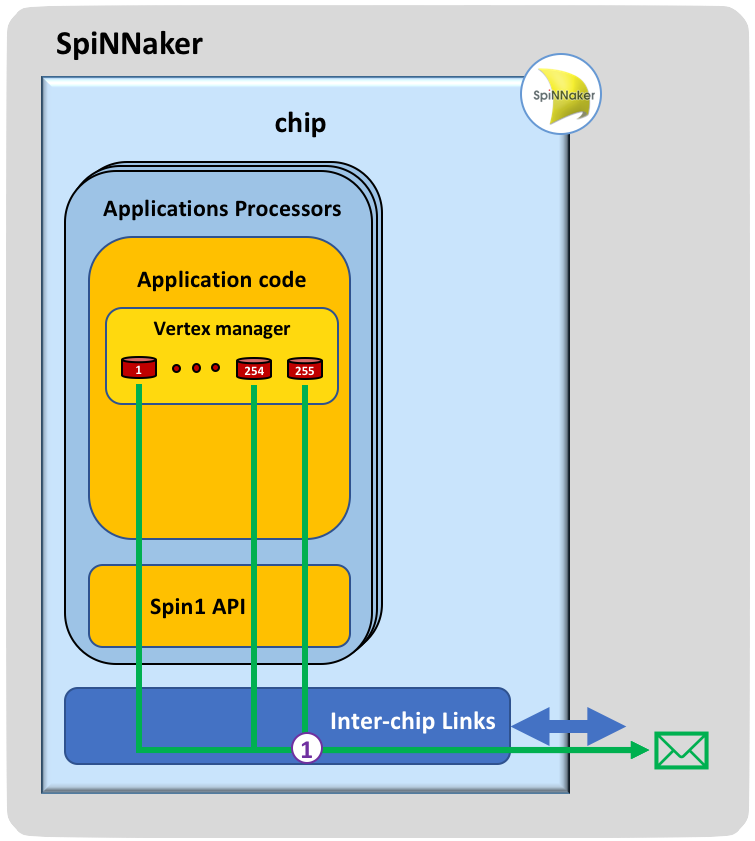
\includegraphics[width=0.82\hsize]{figures/impl-dataflow-out.png}
\caption{Data-flow of outbound messages in Page Rank under SpiNNaker.}
\label{fig:dataflow-out}
\end{figure}

The second step of the computation is more complex, and is related to the reception of inbound packets; see Fig.~\ref{fig:dataflow-in}. The steps described in this figure match the steps ordering described in the section \ref{sec:mplx} about multiplexing / demultiplexing. First, an incoming packet is buffered by the message processor (step 1) while its associated recipient records are loaded from SDRAM via a DMA transfer (step 2). Upon completion (step 3), the message dispatcher is called with the packet key / payload (green) and the loaded records (white) which are used to distribute the message to the specified Page Rank vertices (step 4).

\begin{figure}[hbtp]
\centering 
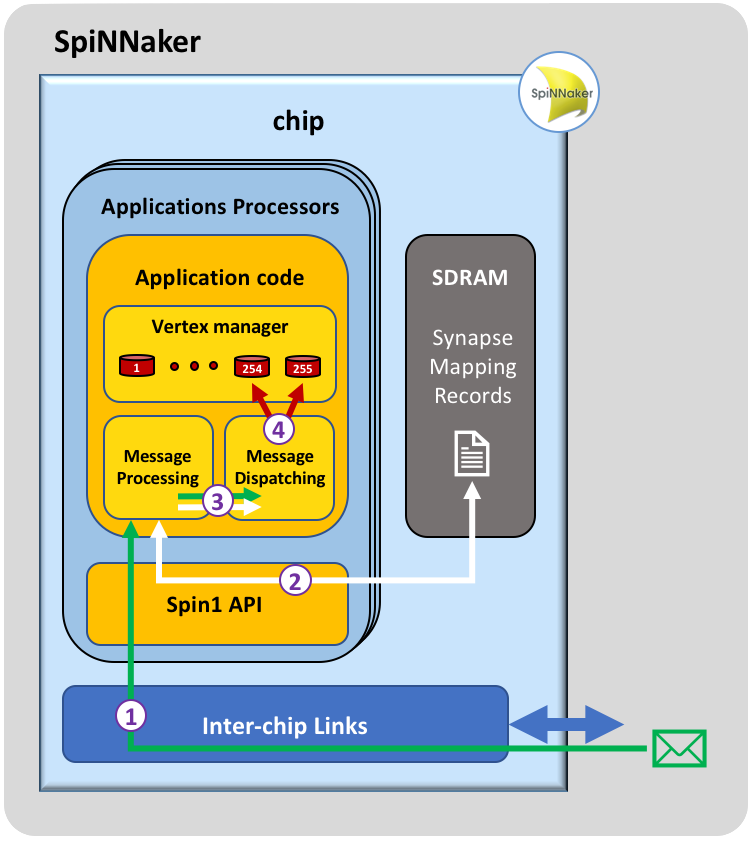
\includegraphics[width=0.9\hsize]{figures/impl-dataflow-in.png}
\caption{Data-flow of inbound messages in Page Rank under SpiNNaker.}
\label{fig:dataflow-in}
\end{figure}

Here again, this message processing strategy is derived from the original spike processing logic in \texttt{sPyNNaker}. Adapting an existing implementation that has proven its robustness through years of operations was an invaluable asset that made an efficient implementation of Page Rank possible. \\ 

Let us now review how iterations are synchronised in a world where there is no such thing as a synchronisation barrier. Indeed, neither the \texttt{Spin1} API nor the \texttt{SARK} library provide a way to globally synchronise all the cores across the system.

\paragraph{Locally synchronous, globally asynchronous}

In Page Rank, the results are computed iteratively one iteration after the other until a convergence point it reached. On a traditional single-threaded implementation, this is simply achieved by executing each iteration one after the other. On a traditional multi-threaded implementation, this is done by having a synchronisation barrier to wait for all workers to complete an iteration before moving to the next one. In SpiNNaker, there are no synchronisation barrier so it was decided to choose a locally synchronous, globally asynchronous approach. \\

Locally, each core waits for all its vertices to complete their iteration before moving to the next one, synchronously as a group. In practice, this is done by using the semaphore API provided by SARK, by having each vertex raise the semaphore at the beginning of the iteration and lower it when it has received all its expected packets. \\
 
Globally, cores are not synchronised and move at their own pace. In that setting, it is possible to have some packets that arrive early, sent by a core that is a few iterations ahead. To cope with this issue, all packets are tagged by the sender with an iteration number, and the receiver maintains distinct per-iteration buffers. Consequently, early packets are buffered until the core advances to the right iteration. Since a core only moves to the next iteration when \textit{all} its vertices have received \textit{all} their expected packets, these cross-core data flow dependencies should ensure (particularly on dense networks) that all cores progress approximately at the same pace. This reduces the need for an exhaustive list of buffers covering each iteration of the simulation; a cycling iteration time stamp of 4 iterations is sufficient in practice. \\

Overall, this implementation achieves good performance speed-ups, which are detailed in section \ref{sec:eval}, and allows Page Rank to scale at a minimal overhead.

\paragraph{Mitigating communication deadlocks}

Finally, a last corner case this implementation mitigates is communication deadlock; an example is visually described in Fig.~\ref{fig:pkt}. Indeed, if a packet is lost by the network, then its recipients could wait for its arrival indefinitely, blocking the entire computation. 

\begin{figure}[hbtp]
\centering 
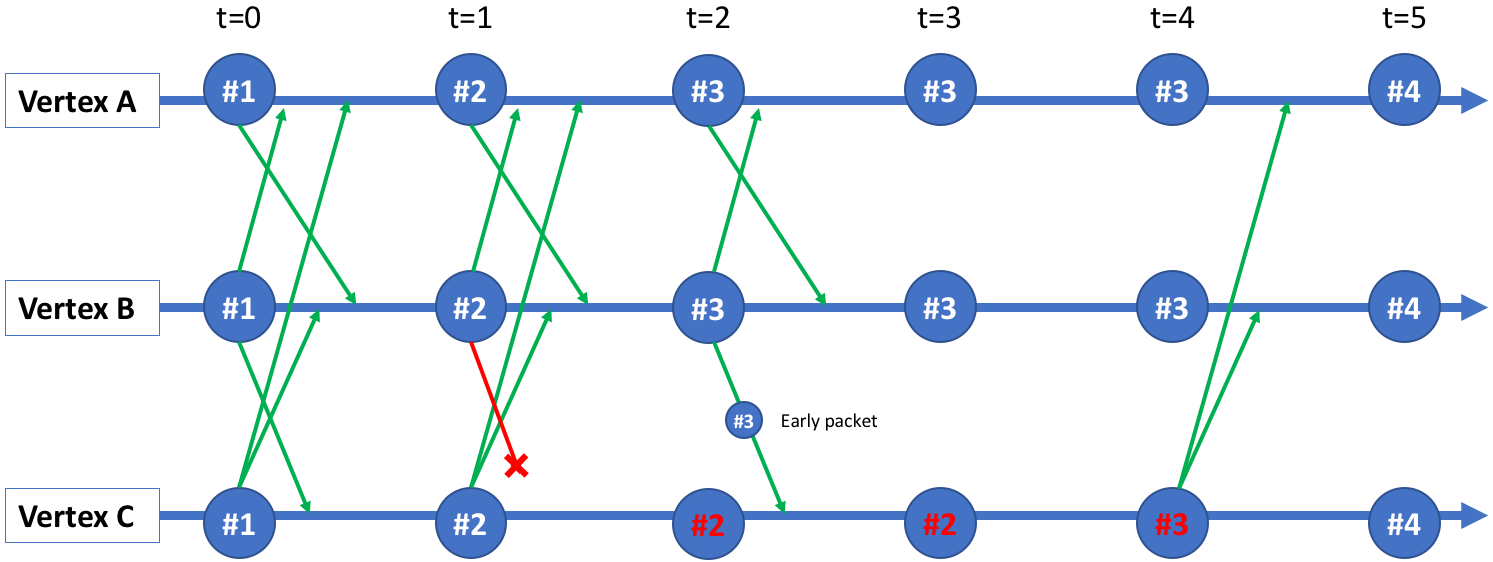
\includegraphics[width=1\hsize]{figures/packet_drop.png}
\caption{Data-flow diagram of packet loss and recovery in the globally asynchronous Page Rank model. This assumes each graph node (i.e. vertex) is on a different core.}
\label{fig:pkt}
\end{figure}

To cope with this issue, a time-out is included at the vertex manager level to force the next iteration if no change has occurred in the vertices' states for over 3 time steps. This threshold was chosen arbitrarily and requires tuning. Let us take the example from Fig.~\ref{fig:pkt}, which assumes all three graph vertices are on different SpiNNaker cores. We notice a packet is dropped during iteration at $t=1$ and causes a communication deadlock. Indeed, vertex C is still expecting a packet from iteration \#2 and vertices A et B wait for a packet from iteration \#3. We also notice an early packet reaches C, which does not cause a problem as the asynchronous model buffers early packets. At the third idle hardware time step at $t=4$, C detects it has deadlocked and forces the next iteration by resetting its state values to their content at the beginning of iteration \#2. It also sends its packets for iteration \#3 right away to A and B. At this point, all vertices have received the necessary packets for iteration \#3 and can move together to the next iteration. \\

However, this solution is quite fragile for two reasons: 

\begin{itemize}
\item The values computed are not correct anymore, since vertex C used old values from iteration \#2 for its iteration \#3. However, near-perfect solutions are still relevant for Page Rank so it is probably tolerable to have a minor level of noise in some outputs. Moveover, the simulation would then continue and converge, most likely erasing gradually the errors from the early stages.

\item Secondly, in the most likely case, A and B will have received updates at time $t=2$, like in this example, meaning their time-out would only occur at time $t=5$. This works correctly as the time-out will occur one step earlier on C, which will send its packet before iteration \#5 begins on A and B. However, if one of these vertices, say A, was only expecting an edge from C, than its time-out would have occurred at time $t=4$. This would have created a new deadlock phase centred around vertex A, and on larger graphs this could result into chains of time-outs that the simulation would not recover from.
\end{itemize}


Nonetheless, it can still allow the computation to recover from a few dropped packets, so it is kept for that purpose.
%EXPLAIN Sample 4 nodes exmaple


\subsection{Correctness considerations} \label{sec:resval}


To validate the correctness of the implementation above, a Python implementation was jointly used to verify the Page Rank results obtained on SpiNNaker. Comparing these results in that setting proved to be too imprecise, as SpiNNaker only supports fixed-point arithmetic operations while Python's floating-point representation is significantly more precise. Consequently, to ensure results would match to the exact bit, a binary fixed-point arithmetic library had to be used to re-implement the Python Page Rank implementation. \\

Additionally, since any remote automated testing (on a continuous integration platform for instance) is hardly doable without the physical board, we opted for local robustness testing. A performance testing script was made to generate arbitrary large graphs and run Page Rank computations on it, verifying each time the results with the Python implementation. This script was run before pushing any commit, and provided a local solution to have a minimal continuous assessment of the correctness of the implementation. \\

Finally, it is noteworthy to mention that \texttt{sPyNNaker} provides a way of collecting monitoring data from simulations. For instance, it counts the number of packets dropped by the network or by an overloaded core, which will be some valuable information for the evaluation section that follows.

%
%Can inspect the machine post-execution, so you know if you dropped some packets at some point. Guaranties you have the right results if no such error message
%
%Routing / chip, so if you make sure each Page Rank vertex is connected to at least another vertex on each of the 4 chips, you maximise the number of packets sent. Robustness tests (and everything in the evaluation section to follow) ran with 10 edges per vertex, ensuring an overwhelming probability that all nodes will be connected to another node of each chip.
%
%TODOs:
%	Exploited graph processing bencharmarks. However, they rely on generic graph processing algorithms whereas we can only run Page Rank for now.
